\chapter{Présentation du projet}
\section{Sujet}
Le problème à N-corps consiste à calculer le mouvement de  $N$ particules en connaissant leur position et leur vitesse initiales respectives.
Il s'agit donc de résoudre les équations du mouvement de Newton pour ces $N$ particules.
Le problème à N-corps est une simulation classique et importante pour l'astronomie, étant donné qu'il permet d'étudier la mécanique de corps célestes interagissant gravitationnellement.
Le problème à deux corps et le problème à trois corps sont résolubles de manière exacte mais ces solutions sont peu efficaces, quant au problème à $4$ corps, il ne possède pas de solution exacte sans postulat supplémentaire. Pour $N>4$, il n'existe pas de résolution exacte, il faut donc utiliser des solutions approchées.

%inclusion d'une mage dans le document
\begin{figure}[!h]
\begin{center}
%taille de l'image en largeur
%remplacer "width" par "height" pour régler la hauteur
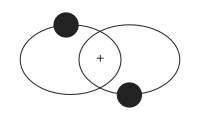
\includegraphics[scale=0.8]{presentation/two.png}
%légende de l'image
\captionsetup{hypcap=false}
\caption{Solution du problème à 2 corps \\
source : \url{https://www.chegg.com}}
\label{fig1}
\end{center}
\end{figure}

\section{Objectif : résolution la plus efficace possible du problème à N-corps}

L'objectif du projet est donc de résoudre le plus efficacement possible le problème à N-corps afin de simuler des galaxies.
Il sera alors intéressant de comparer les performances de ces méthodes.
Pour cela, nous utiliserons des solutions approchées calculées à partir de différents algorithmes dont l'algorithme de Barnes-Hut. Nous étudierons également l'application de la parallélisation à notre programme.
En pratique, le projet consiste à compléter et améliorer un projet déjà commencé afin d'acquérir de nouvelles compétences en C++, sur les algorithmes hiérarchiques, en parallélisation et plus généralement en optimisation de code.

\section{Démarche}

Pour chaque particule, il est nécessaire de calculer la force gravitationnelle qui s'y applique puis d'utiliser un intégrateur numérique pour calculer sa position. Pour le calcul des forces, il est alors intéressant d'utiliser différents algorithmes notamment le calcul naïf et l'algorithme de Barnes-Hut. Pour l'intégration, il est possible d'utiliser la méthode d'Euler ou la méthode saute mouton.
Par la suite, il sera intéressant d'explorer les différentes possibilités d'optimisation, telle que la parallélisation multi-thread. 